\documentclass{article}
\usepackage[a4paper, total={6.5in, 10in}]{geometry}
\usepackage[utf8]{inputenc}
\usepackage[T1]{fontenc}
\usepackage{polski}
\usepackage{amsfonts}
\usepackage{graphicx}
\usepackage{enumitem}

\title{WSYZ kolokwium 2 - rozwiązania}
\author{Jakub Ostrzołek}

\begin{document}
\maketitle

\section*{Zadanie 1.}

\subsection*{Oznaczenia}
\begin{itemize}
	\item $t_J \in \mathbb{N}$ - liczba godzin pracy Janusza
	\item $t_G \in \mathbb{N}$ - liczba godzin pracy Grzegorza
\end{itemize}

\subsection*{Warunki}
$$0 \le t_J \le 7$$
$$0 \le t_G \le 8$$

$$t_J + t_G \le 12$$
$$t_G \le t_J$$

\subsection*{Funkcja celu}
$$\max{(t_J \cdot 4 + t_G \cdot 3)}$$

\subsection*{Rozwiązanie graficzne}
\begin{center}
	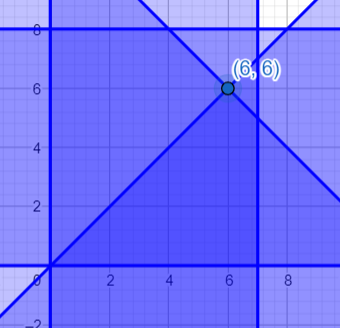
\includegraphics{zad1.png}
\end{center}

\pagebreak
\section*{Zadanie 2.}

Przykładowy harmonogram
\begin{verbatim}
	   0000000001111111
	   1234567891234567
	A: XXXXX,,,,,,,,,,,
	B: ##,,,,,,,,,,,,,,
	C: ,,,,,####,,,,,,,
	D: ,,,,,###,,,,,,,,
	E: ,,,,,,,,,####,,,
	F: ,,,,,XXXXXXXXXXX
	G: ,,,,,#########,,
\end{verbatim}

\begin{enumerate}[label=\alph*)]
	\item $T_{min}= 17$

	      Zapasy całkowite
	      \begin{itemize}
		      \item $\Delta t_B = 3$
		      \item $\Delta t_D = 4$
	      \end{itemize}

	      Zapasy swobodne
	      \begin{itemize}
		      \item $\Delta t_B' = 3$
		      \item $\Delta t_D' = 1$
	      \end{itemize}
	\item
	      \begin{verbatim}
			   0000000001111111
			   1234567891234567
			A: XXXXX,,,,,,,,,,,
			B: ,,,##,,,,,,,,,,,
			C: ,,,,,####,,,,,,,
			D: ,,,,,,###,,,,,,,
			E: ,,,,,,,,,####,,,
			F: ,,,,,XXXXXXXXXXX
			G: ,,,,,#########,,
		   \end{verbatim}
\end{enumerate}

\section*{Zadanie 3.}
Reguła SPT \emph{(Shortest Processing Time)}.

Z4 $\rightarrow$
Z7 $\rightarrow$
Z1 $\rightarrow$
Z6 $\rightarrow$
Z10 $\rightarrow$
Z8 $\rightarrow$
Z2 $\rightarrow$
Z5 $\rightarrow$
Z9 $\rightarrow$
Z3

\section*{Zadanie 4.}
\subsection*{Model sieci przepływowej}
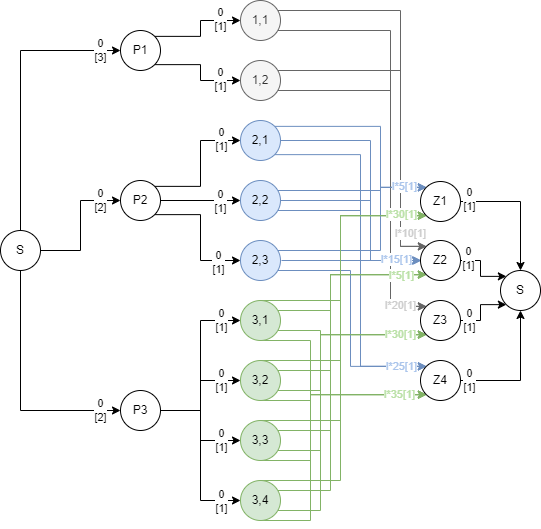
\includegraphics[height=0.4\paperheight]{zad4.png}

Zadany przepływ to $F=4$.

\subsection*{Model programowania liniowego}
\subsubsection*{Zbiory}
\begin{itemize}
	\item $Z = {1, 2, 3, 4}$ - zadania
	\item $P = {1, 2, 3}$ - procesory
\end{itemize}

\subsubsection*{Zmienne}
\begin{itemize}
	\item $p_{jkl} \in \{0, 1\}$ - czy zadanie j wykonuje się na procesorze k na miejscu l-tym od końca
\end{itemize}

\subsection*{Ograniczenia}
$$\forall j \in Z, k \in P: \; \sum_{l \in Z} p_{jkl} \le 1$$
$$\sum_{j \in Z, l \in Z} p_{j1l} \le 3 $$
$$\sum_{j \in Z, l \in Z} p_{j2l} \le 2 $$
$$\sum_{j \in Z, l \in Z} p_{j3l} \le 2 $$
$$\forall j \in \{1, 4\}, l \in Z: \; p_{j1l} = 0$$
$$\forall j \in \{3\}, l \in Z: \; p_{j1l} = 0$$
$$\forall j \in Z: \; \sum_{k \in P, l \in Z} p_{jkl} = 1$$

\subsection*{Funkcja celu}
$$\min{\sum_{l \in Z} l \cdot (
		p_{12l} \cdot 10 +
		p_{13l} \cdot 20 +
		p_{21l} \cdot 5 +
		p_{22l} \cdot 15 +
		p_{24l} \cdot 25 +
		p_{31l} \cdot 30 +
		p_{32l} \cdot 5 +
		p_{33l} \cdot 30 +
		p_{34l} \cdot 35
		) / 4}$$

\end{document}